\chapter{Desenvolvimento}

Esta seção tem como objetivo apresentar o processo de desenvolvimento da proposta atual, fundamentado nas etapas previamente descritas na seção de metodologia. Serão discutidos também os desafios encontrados durante o processo e possíveis ajustes na direção do projeto à medida que obstáculos emergem.

O processo de desenvolvimento da proposta inicia com a etapa de Mapeamento, na qual serão definidos os requisitos, formuladas as perguntas de pesquisa, realizado o mapeamento sistemático da literatura e estabelecidos os requisitos não funcionais para acessibilidade.

Em seguida, na etapa de Modelagem, serão construídos o Diagrama de Sequência, o Diagrama de Componentes, o Modelo Lógico de Dados e o Diagrama de Classes. Esses diagramas e modelos servirão como alicerce para a próxima fase.

Na fase do Projeto, será projetada a arquitetura de integração com o Flutter e selecionados os frameworks, bibliotecas e linguagens que serão usados no desenvolvimento da ferramenta.

Com a conclusão da etapa de Projeto, o processo de Desenvolvimento será iniciado, onde serão aplicados Padrões de Projeto e Expressões regulares, além de preparar a ferramenta para publicação.

Após a conclusão do desenvolvimento, a etapa de Testes será iniciada. Nela, será adotado o TDD, serão realizados Testes de Unidade e de Integração, bem como Testes dos Requisitos não funcionais de Acessibilidade.

Finalmente, na etapa de Validação, será realizada uma pesquisa com desenvolvedores e pessoas com deficiência, aplicado o SUS e executada uma prova de conceito. Essa etapa final permitirá avaliar a eficácia da ferramenta desenvolvida e identificar áreas de melhoria potencial. Cada uma dessas etapas será discutida em detalhes nas seções subsequentes deste capítulo.

\section{Mapeamento Inicial}

O processo inicial de mapeamento é fundamental para a abordagem de identificação dos Requisitos Funcionais (RF), Requisitos Não Funcionais (RNF) e Regras de Negócio (RN).

Os Requisitos Funcionais (RF) são destinados a descrever as funcionalidades que o sistema deve incorporar para atender às necessidades do usuário final. Estes requisitos são essencialmente as ações que o sistema deve ser capaz de realizar, como por exemplo, processar entradas de dados, realizar operações e fornecer saídas de informações.

Por outro lado, os Requisitos Não Funcionais (RNF) definem o conjunto de critérios que orientam o modo como o sistema operará, como as restrições e propriedades desejáveis do sistema que não estão diretamente relacionadas com o comportamento específico dele. Eles estabelecem um escopo com características particulares que o sistema a ser desenvolvido deverá seguir, tais como padrões de projeto, usabilidade, segurança, desempenho, entre outros. Em outras palavras, os RNF são os atributos de qualidade do sistema que determinam como os requisitos funcionais devem ser implementados.

As Regras de Negócio (RN), por sua vez, são diretrizes que definem ou restringem algum aspecto do negócio. Elas descrevem os detalhes das funcionalidades que o sistema deve possuir, para que estas possam ser implementadas de forma a não causar prejuízos a outras funcionalidades. Elas fornecem uma compreensão clara de como o sistema deve se comportar em determinadas circunstâncias e auxiliam na garantia de que o sistema esteja alinhado com as metas e estratégias do negócio.

Em suma, a identificação e compreensão desses três elementos - RF, RNF e RN - são cruciais para o sucesso do desenvolvimento do sistema, garantindo que ele seja construído de acordo com as necessidades do negócio e dos usuários, além de cumprir com os critérios de qualidade estabelecidos.

\subsection{Requisitos Funcionais}

Os Requisitos Funcionais (RF) identificados para o sistema proposto são:

\newcounter{rf} 
\renewcommand{\therf}{RF\arabic{rf}}

\begin{table}[!htbp]
	\centering
	\renewcommand{\arraystretch}{1.1}
	\caption{Requisitos Funcionais do TCC}
	\label{tab:tabela-requisitos-funcionais}
	\begin{tabular}{ L{2cm}  L{12cm} }
		\hline
		Requisito & Descrição \\
		\hline
		\refstepcounter{rf}\therf	& O sistema deve analisar código escrito na linguagem Dart \\
    \refstepcounter{rf}\therf	& O sistema deve possuir requisitos não funcionais voltados a acessibilidade \\
    \refstepcounter{rf}\therf	& O sistema deve permitir a visualização de inconsistências no código \\
    \refstepcounter{rf}\therf	& O sistema deve realizar marcações no código baseado na especificação definida \\
    \refstepcounter{rf}\therf	& O sistema deve sugerir remover trechos de código baseado na especificação definida \\
    \refstepcounter{rf}\therf	& O sistema deve sugerir correções automáticas baseado na especificação definida \\
    \refstepcounter{rf}\therf	& O sistema deve permitir o usuário consultar todas as baseado os requisitos não funcionais de acessibilidade \\
    \refstepcounter{rf}\therf	& O sistema deve permitir o usuário desabilitar requisitos não funcionais de acessibilidade \\
    \refstepcounter{rf}\therf	& O sistema deve permitir a utilização em ambientes de integração contínua \\

		\hline
	\end{tabular}
	\vspace{2mm}
	\fonte{\me{2023}}
\end{table}

Dos requisitos funcionais da tabela \ref{tab:tabela-requisitos-funcionais}, destaca-se a necessidade de analisar código escrito na linguagem Dart, isso depende de uma ferramenta capaz de processar e interpretar o código fonte da aplicação desenvolvida com Flutter. A equipe do Dart provê uma API para análise estática de código, que será utilizada através do plugin \href{https://pub.dev/packages/analyzer}{analyzer}. Ele já provê uma interface para acessar a árvore sintática abstrata do código fonte, que será utilizada para identificar e marcar as inconsistências no código.

\subsection{Requisitos Não Funcionais}

Os Requisitos Não Funcionais (RNF) identificados para o sistema proposto são:

\newcounter{rnf}
\renewcommand{\thernf}{RNF\arabic{rnf}}

\begin{table}[!htbp]
	\centering
	\renewcommand{\arraystretch}{1.1}
	\caption{Requisitos Não Funcionais do TCC}
	\label{tab:tabela-requisitos-nao-funcionais}
	\begin{tabular}{ L{2cm}  L{12cm} }
		\hline
		Requisito & Descrição \\
		\hline
		\refstepcounter{rnf}\thernf	& O sistema deve ser escrito utilizando a linguagem Dart \\
		\refstepcounter{rnf}\thernf	& O sistema deve ser publicado no repositório \href{https:\\pub.dev}{pub.dev} \\
		\refstepcounter{rnf}\thernf	& O sistema deve seguir as melhores práticas para pacotes publicados no repositório \href{https:\\pub.dev}{pub.dev} \\
    \refstepcounter{rnf}\thernf	& O sistema deve possuir licença aberta para permitir alterações e melhorias \\
    \refstepcounter{rnf}\thernf	& O sistema deve possuir documentação para auxiliar na criação de novas regras de negócio de usabilidade \\
		\hline
	\end{tabular}
	\vspace{2mm}
	\fonte{\me{2024}}
\end{table}

Dos requisitos funcionais descritos na tabela \ref{tab:tabela-requisitos-nao-funcionais}, destaca-se a necessidade de seguir as melhores práticas para pacotes publicados no repositório \href{https:\\pub.dev}{pub.dev}. Isso é importante para garantir que o sistema seja facilmente acessível e utilizável por outros desenvolvedores, além de manter a qualidade e a segurança do código fonte. A equipe do Dart provê um guia de boas práticas para publicação de pacotes no repositório \href{https:\\pub.dev}{pub.dev}, que será seguido para garantir a qualidade e a segurança do sistema. Ele também é uma das formas que o repositório classifica plugins auxiliando na escolha dos usuários.

\subsection{Regras de Negócio}

As Regras de Negócio (RN) identificadas para o sistema proposto são:

\newcounter{rn} 
\renewcommand{\thern}{RN\arabic{rn}}

\begin{table}[!htbp]
	\centering
	\renewcommand{\arraystretch}{1.1}
	\caption{Regras de negócio do TCC}
	\label{tab:tabela-regras-de-negocio}
	\begin{tabular}{ L{2cm}  L{12cm} }
		\hline
		Regra de Negócio & Descrição \\
		\hline
		\refstepcounter{rn}\thern	& As regras de acessibilidade devem ser separadas por pastas para organização clara e simplificada \\
    \refstepcounter{rn}\thern	& Cada regra de acessibilidade deve possuir testes automatizados para validar seu funcionamento \\
    \refstepcounter{rn}\thern	& Cada regra de acessibilidade deve possuir uma descrição clara e objetiva para facilitar a compreensão do desenvolvedor \\
    \refstepcounter{rn}\thern	& Cada regra de acessibilidade deve possuir uma sugestão de correção \\
    \refstepcounter{rn}\thern	& Cada regra de acessibilidade deve possuir uma marcação no código para indicar a inconsistência \\
    \refstepcounter{rn}\thern & As marcações devem ser na cor Laranja, uma vez que a cor vermelha é utilizada para erros de compilação \\
		\hline
	\end{tabular}
	\vspace{2mm}
	\fonte{\me{2024}}
\end{table}

Além das regras de negócio listadas na tabela \ref{tab:tabela-regras-de-negocio}, destaca-se a necessidade de separar as regras de acessibilidade por pastas para organização clara e simplificada. A ideia inicial era utilizar um Mapeamento Sistemático da Literatura para identificar as regras de acessibilidade mais utilizadas e criar um conjunto de regras de acessibilidade padrão. Porém, conforme será descrito nos próximos capítulos, não foi possível levantar um conjunto de regras de acessibilidade padrão, então optou-se por criar um conjunto de regras de acessibilidade baseado nas recomendações de ambas as plataformas.

\section{Modelagem}

Com os requisitos identificados, a próxima etapa é a Modelagem, onde serão construídos os diagramas e modelos que servirão como base para o desenvolvimento do sistema.

\subsection{Diagrama de Sequência}

Diagramas de sequência são diagramas de interação que mostram como grupos de objetos colaboram em algum comportamento ao longo do tempo. Eles são usados para capturar o comportamento de um único caso de uso, ou seja, um cenário específico de interação entre objetos.

O diagrama de sequência da figura \ref{fig:diagrama-sequencia-plugin} a seguir ilustra a interação básica do desenvolvedor com o plugin:

\begin{figure}[!h]
	\centering
	\caption{Interação do desenvolvedor com o plugin}\label{fig:diagrama-sequencia-plugin}
	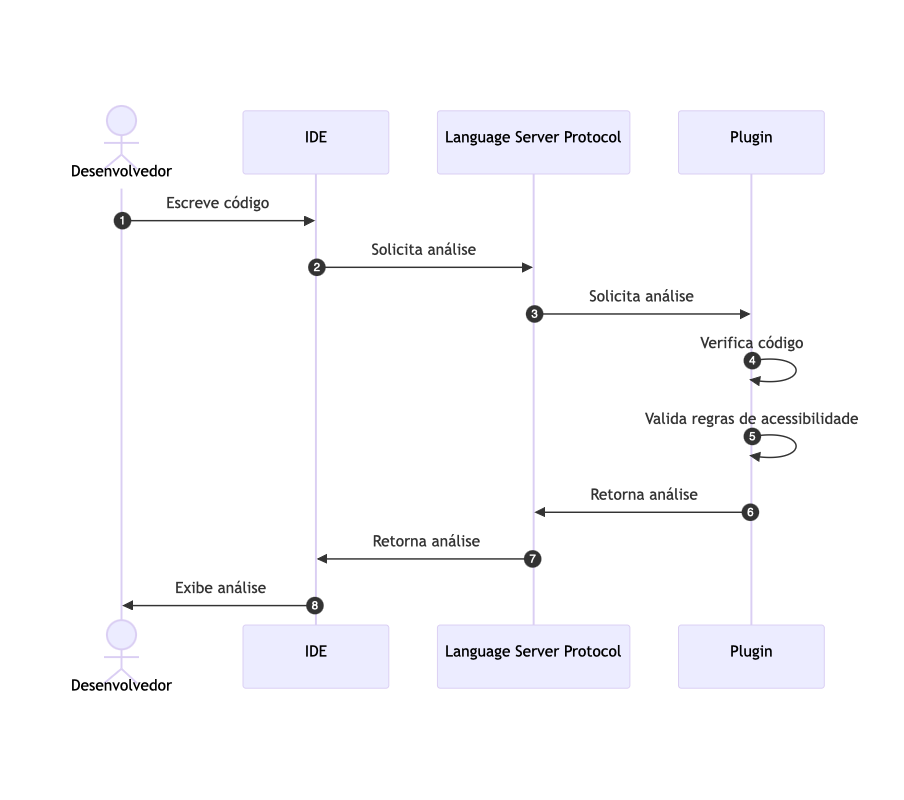
\includegraphics[width=325pt]{Assets/DiagramaSequenciaIDELSPPlugin.png}
	\fonte{\me{2024}}
\end{figure}

Como podemos ver na figura \ref{fig:diagrama-sequencia-plugin}, o desenvolvedor interage com o plugin através da IDE, que por sua vez executa a análise estática do código fonte da aplicação desenvolvida com Flutter. O plugin então marca o código fonte baseado nas regras de acessibilidade definidas e sugere correções automáticas. Isso torna todo o processo de desenvolvimento mais eficiente e permite que regras de acessibilidade sejam aplicadas desde o início do desenvolvimento sem a necessidade de compilar e executar a aplicação.

Entretanto o diagrama da figura \ref{fig:diagrama-sequencia-plugin} não mostra a interação do plugin com as regras de acessibilidade, para isso foi criado o diagrama de sequência da figura \ref{fig:diagrama-sequencia-regra-acessibilidade}:

\begin{figure}[!h]
  \centering
  \caption{Interação do plugin com as regras de acessibilidade}\label{fig:diagrama-sequencia-regra-acessibilidade}
  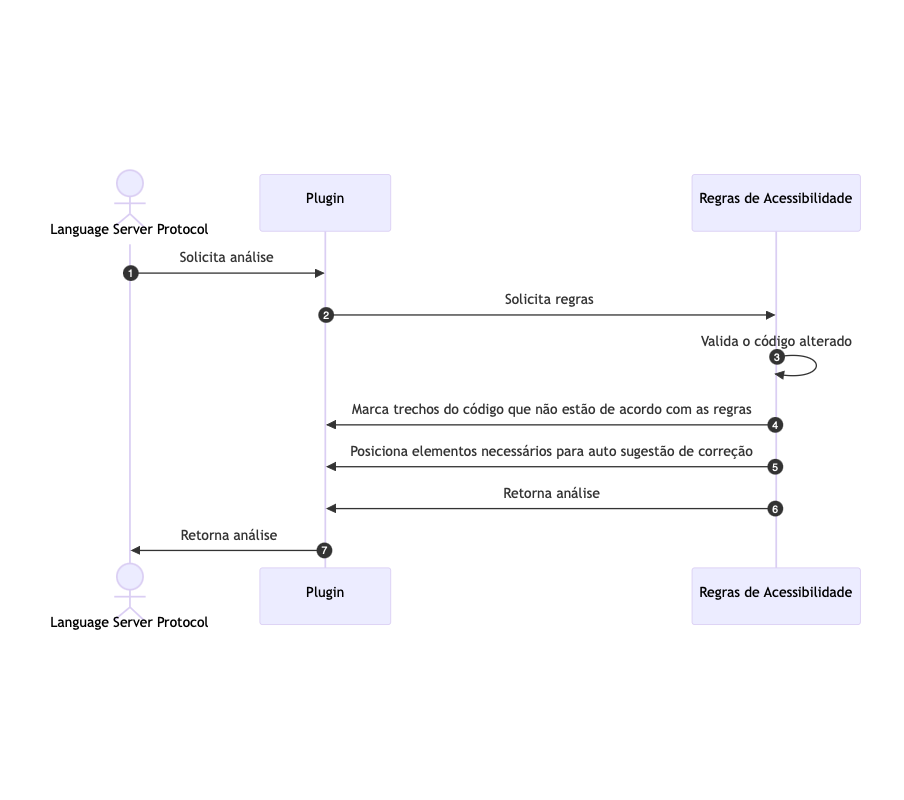
\includegraphics[width=325pt]{Assets/DiagramaPluginRegrasAcessibilidade.png}
  \fonte{\me{2024}}
\end{figure}

Como é possível identificar na figura \ref{fig:diagrama-sequencia-regra-acessibilidade}, o ponto de partida é o LSP que envia o código fonte do desenvolvedor para o Plugin, que então irá processar o código fonte aplicando todas as regras de acessibilidade definidas de uma forma sequencial. Cada regra de acessibilidade é aplicada ao código fonte e, caso uma inconsistência seja encontrada, o plugin marca o código fonte e sugere correções automáticas.

Um dos requisitos é ser possível utilizar o plugin através de uma linha de comando possibilitando integração com ambientes de integração contínua, para isso foi criado o diagrama de sequência da figura \ref{fig:diagrama-sequencia-linha-comando}:

\begin{figure}[!h]
	\centering
	\caption{Interação do plugin com a linha de comando}\label{fig:diagrama-sequencia-linha-comando}
	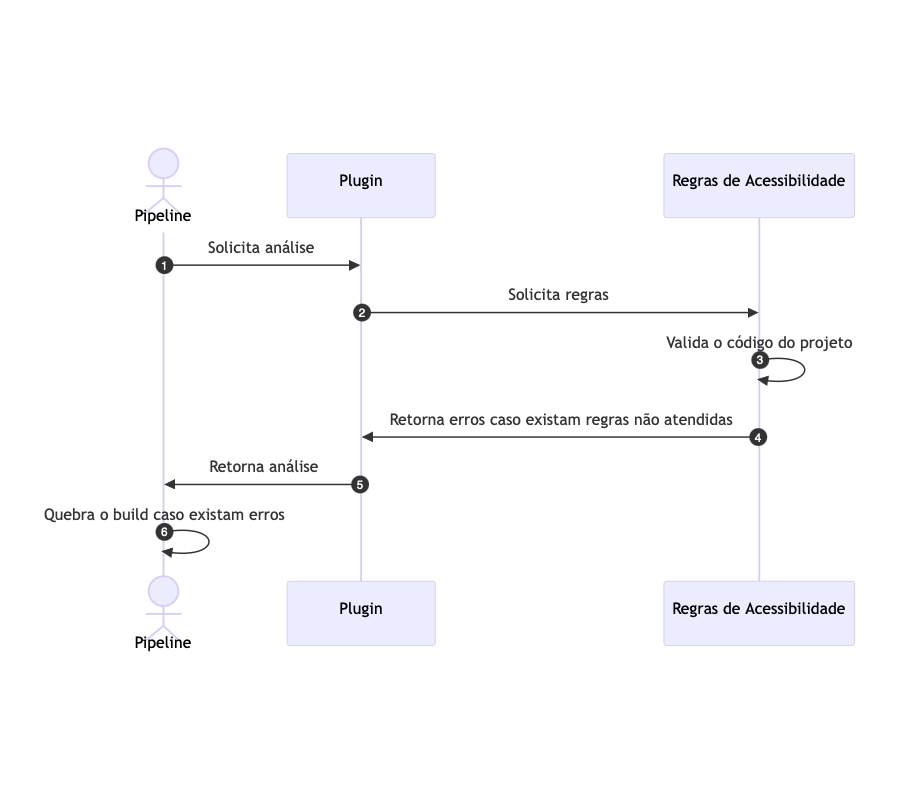
\includegraphics[width=325pt]{Assets/DiagramaSequenciaLinhaComando.png}
	\fonte{\me{2024}}
\end{figure}

O principal objetivo de integrar o plugin em ambientes de integração contínua é garantir que as regras de acessibilidade sejam aplicadas em todas as fases do desenvolvimento, desde a escrita do código até a compilação e execução da aplicação. Isso permite que os desenvolvedores travem a publicação de aplicações que não atendam aos requisitos de acessibilidade, garantindo que todas as aplicações desenvolvidas com Flutter sejam acessíveis a todos os usuários.

\subsection{Provas de Conceito}

\subsubsection{Extensão para Visual Studio Code}

Na concepção do projeto, a ideia era criar uma extensão para Visual Studio Code capaz de realizar a análise estática de código Dart e Flutter e retornar ao usuário as regras de acessibilidade que não foram seguidas. Porém, durante o desenvolvimento, percebeu-se que a seria necessário desenvolver toda uma infraestrutura de análise estática de código, o que demandaria muito tempo e recursos. Além disso, a equipe do Dart já provê uma API para análise estática de código, que será utilizada através do plugin \href{https://pub.dev/packages/analyzer}{analyzer}. 

Ademais, uma implementação focada em Visual Studio Code limitaria o alcance do projeto, uma vez que a extensão seria específica para essa IDE. Por isso, optou-se por desenvolver um plugin para LSP, que é uma interface de comunicação entre a IDE e o plugin, permitindo que o plugin seja utilizado em qualquer IDE que suporte LSP. Porém, ainda assim esbarra-se na necessidade de desenvolver uma infraestrutura de análise estática de código, o que demandaria muito tempo e recursos.

\subsubsection{Extensão para DevTools do Flutter}

DevTools é uma ferramenta de diagnóstico para Flutter que permite visualizar e inspecionar o comportamento da aplicação em execução. A ideia era criar uma extensão para DevTools capaz de realizar a análise estática de código Dart e Flutter e retornar ao usuário as regras de acessibilidade que não foram seguidas. Tal implementação seria agnóstica de IDE e uma vez que desenvolvida em Dart, poderia utilizar o pacote \href{https://pub.dev/packages/analyzer}{analyzer} para realizar a análise estática de código e processar o código fonte da aplicação desenvolvida com Flutter.

Porém, tal abordagem não seria capaz de marcar o código fonte da aplicação desenvolvida com Flutter, uma vez que DevTools é uma ferramenta de diagnóstico e não uma IDE. Sendo assim, tal ideia foi descartada após a realização de alguns testes.

\subsubsection{Plugin para Dart utilizando o pacote \href{https://pub.dev/packages/analyzer_plugin}{analyzer\_plugin}}

Haja vista que o projeto visava criar um plugin agnóstico de IDE porém ainda capaz de se comunicar com LSP tornando possível a marcação, sugestão de correção e validação de regras de acessibilidade, foi decidido utilizar o pacote \href{https://pub.dev/packages/analyzer_plugin}{analyzer\_plugin} para criar um plugin para Dart. O pacote \href{https://pub.dev/packages/analyzer_plugin}{analyzer\_plugin} é uma API para criar plugins para o Dart Analysis Server, que é uma ferramenta de análise estática de código Dart.

Seguindo a documentação oficial do pacote, foi então iniciado o desenvolvimento de uma prova de conceito. Para isso, foi então criado um novo projeto em Dart utilizando o template de pacote. Esse template estrutura um projeto Dart com uma base ideal para o desenvolvimento de um pacote que possa ser posteriormente publicado no repositório \href{https://pub.dev}{pub.dev}.

Para tal é necessário executar o seguinte comando: \texttt{dart create -t package-simple <nome\_do\_projeto>} que após a execuçaõ, irá gerar uma estrutura similar a apresentada a seguir:

\begin{verbatim}
<nome_do_projeto>
	CHANGELOG.md
	README.md
	analysis_options.yaml
	example/
		<nome_do_projeto>_example.dart
	lib/
		<nome_do_projeto>.dart
		src/
			<nome_do_projeto>_base.dart
	pubspec.lock
	pubspec.yaml
	test/
		<nome_do_projeto>_test.dart
\end{verbatim}

Com o projeto base criado, é então necessário adicionar as dependências necessárias para o desenvolvimento do plugin. Para isso, foi necessário executar o seguinte comando: \texttt{dart pub add analyzer\_plugin analyzer} que irá adicionar a dependência do pacote \href{https://pub.dev/packages/analyzer_plugin}{analyzer\_plugin} e do pacote \href{https://pub.dev/packages/analyzer}{analyzer} ao arquivo \texttt{pubspec.yaml}. Ambos são pacotes oficiais do time do Dart.

Seguindo então a documentação do \cite{documentacaoanalyzerplugin} foi possível chegar em uma implementação capaz de avaliar código fonte escrito em Dart e retornar as regras de acessibilidade que não foram seguidas. Entretanto a falta de suporte da equipe para com o pacote \href{https://pub.dev/packages/analyzer_plugin}{analyzer\_plugin} fez com que a implementação fosse abandonada. 

As principais dificuldades encontradas foram: 

\begin{itemize}
	\item Falta de documentação: A documentação oficial do pacote \href{https://pub.dev/packages/analyzer_plugin}{analyzer\_plugin} é escassa e não cobre todos os aspectos necessários para o desenvolvimento de um plugin para Dart.
	\item Falta de suporte: A equipe do Dart não fornece suporte para o pacote \href{https://pub.dev/packages/analyzer_plugin}{analyzer\_plugin}, o que torna difícil encontrar soluções para problemas específicos.
	\item Complexidade: O pacote \href{https://pub.dev/packages/analyzer_plugin}{analyzer\_plugin} é complexo e requer um conhecimento avançado de Dart e análise estática de código para ser utilizado corretamente.
	\item Falta de integração: O pacote não é capaz de integrar com o analisador padrão do Dart, o que dificulta a implementação de regras de acessibilidade personalizadas. Necessitando que o desenvolvedor que consuma o pacote tenha de executar uma série de comandos para que o plugin funcione corretamente.
\end{itemize}

\subsubsection{Plugin para Dart utilizando o pacote \href{https://pub.dev/packages/custom_lint_builder}{custom\_lint\_builder}}

Após a tentativa frustrada de utilizar o pacote \href{https://pub.dev/packages/analyzer_plugin}{analyzer\_plugin}, foi então decidido utilizar o pacote \href{https://pub.dev/packages/custom_lint_builder}{custom\_lint\_builder} para criar um plugin para Dart. Apesar de ele necessitar que o usuário final importe o pacote \href{https://pub.dev/packages/custom_lint}{custom\_lint} no seu projeto, utilize arquivos diferentes para a personalização de regras de acessibilidade, e também necessitar de uma interface de linha de comando própria, sendo incompatível com o comando \texttt{dart analyze} do Dart, ele é atualmente a melhor opção para a criação de um plugin "linter" para Dart.